%[127~r\textsuperscript{o}] Ebene \edtext{bois}{\lemma{Ebene}\Bfootnote{\textit{(1)} poids \textit{(2)} bois \textit{L}}} fort pesant, sapin, bois fort leger. \textso{P. Pardies\protect\index{Namensregister}{\textso{Pardies}, Ignace Gaston 1636-1673} Statique artic. 14.} ligne de direction du \edtext{Corps du}{\lemma{Corps}\Bfootnote{\textit{(1)} passe d \textit{(2)} du \textit{L}}} Centre de Gravit\'{e} au Centre des \edtext{Graves.}{\lemma{Graves.}\Cfootnote{\textsc{I. G. Pardies}, \cite{00296}a.a.O., S. 17.}} \textso{20} \edtext{\textit{Cette obelisque prodigieuse}}{\lemma{20}\Bfootnote{\textit{(1)} la Grande Ob \textit{(2)} \textit{Cette obelisque prodigieuse} \textit{L}}} \textit{de Rome}\protect\index{Ortsregister}{Rom} \textit{se soutient sur son pied-estal, sans y etre ciment\'{e}e autrement que par son propre poids.} 
\pstart%
[127~r\textsuperscript{o}]
Ebene \edtext{bois}{\lemma{Ebene}\Bfootnote{\textit{(1)} poids \textit{(2)} bois \textit{L}}} fort pesant, sapin, bois fort leger.
\protect\index{Namensregister}{\textso{Pardies}, Ignace Gaston 1636-1673}P. \textso{Pardies \textit{Statique} artic. 14.}
ligne de direction du
\edtext{Corps du}{\lemma{Corps}\Bfootnote{\textit{(1)} passe d \textit{(2)} du \textit{L}}} Centre de Gravit\'{e} au Centre des
\edtext{Graves.}{\lemma{Graves.}\Cfootnote{\textsc{I. G. Pardies}, \cite{00296}a.a.O., S. 17.}}
\pend%
\pstart%
\edtext{\textso{20} \textit{Cette obelisque prodigieuse}}{\lemma{20}\Bfootnote{\textit{(1)} la Grande Ob \textit{(2)} \textit{Cette obelisque prodigieuse} \textit{L}}}
\textit{de Rome}\protect\index{Ortsregister}{Rom} \textit{se soutient sur son pied-estal, sans y etre ciment\'{e}e autrement que par son propre poids.} 
\pend%
\pstart 21 Pictoribus observandum est, ut linea directionibus, nunquam non cadat in basin corporis, alioquin talis positura est \edtext{impossibilis.}{\lemma{impossibilis.}\Cfootnote{\textsc{I. G. Pardies}, \cite{00296}a.a.O., S. 27.}} 
\pend 
\count\Bfootins=1200
\count\Cfootins=1200
\pstart \textso{25} Proposition fondamentalle de la Statique. Corpora sunt in aequilibrio si longitudines brachiorum librae, sunt in ratione ponderum \edtext{reciproca.}{\lemma{reciproca.}\Cfootnote{\textsc{I. G. Pardies}, \cite{00296}a.a.O., S. 31.}} Hoc demonstrat demonstratione quae omnes evitet difficultates demonstrationis \edtext{Archimedeae,}{\lemma{Archimedeae,}\Cfootnote{\textsc{I. G. Pardies}, \cite{00296}a.a.O., S. 40.}} sed dissimulat art. 30. eam demonstrandi rationem deberi ingenio Galilaei\protect\index{Namensregister}{\textso{Galilei} (Galilaeus, Galileus), Galileo 1564-1642}. 
\pend 
\pstart \textso{35} Natura tantundem ponderis in animalibus ab utroque latere locavit, item anteretroque observante quoque \edtext{Galeno.}{\lemma{Galeno.}\Cfootnote{\textsc{I. G. Pardies}, \cite{00296}a.a.O., S. 49.}}\protect\index{Namensregister}{\textso{Galenos} von Pergamon (Aelius Galenus, Claudius Galenus) ca 129-215}
Partes geminae, aeque distant e medio, simplices in medio. Si quae non in medio, ab alterius generis membro compensatur, ita hepar, lien, cor, pulmones, sed et animalia se accommodant corporum naturae. Ventricosi retro se inclinant, at gibbi, et qui onere portant, antrorsum. Si nos inclinamus levandi aliquid causa pedem retrahimus, aut hominum toutes les fesses, alioquin laberemur, cum plus sit ponderis, antrorsum. Hinc nihil remotiosculum elevabis, lorsqu'on met les talons joignant contre une muraille. \textit{De même quand nous tr\'{e}sbouchons, et que nous panchons d'un cost\'{e} sur le point de tomber, nous \'{e}tendons incontinent le bras ou la jambe de l'autre cost\'{e}, afin qu'estant ainsi \'{e}loign\'{e}e au de l\`{a} des pieds ou de la ligne de direction, ils ayent plus de force, pour \edtext{balancer}{\lemma{balancer}\Cfootnote{Bei Pardies contreballancer}} le reste du \edtext{corps.}{\lemma{corps.}\Cfootnote{\textsc{I. G. Pardies}, \cite{00296}a.a.O., S. 51.}}}
\textit{Les oiseaux qui ont un long col, ont aussi des longues jambes, qu'ils estendent en arriere en volant, comme les} \edtext{\textit{cicognes.}}{\lemma{\textit{cicognes.}}\Cfootnote{\textsc{I. G. Pardies}, \cite{00296}a.a.O., S. 52.}} 
\pend 
\pstart
\textso{39} \textit{Nous avons plus de force \`{a} mordre entre les dents du fond des machoires, qu'avec celles de devant la bouche, parce que les machoires se meuuent comme autour d'un centre qui est vers le fond des} \edtext{\textit{machoires.}}{\lemma{\textit{machoires}.}\Cfootnote{\textsc{I. G. Pardies}, \cite{00296}a.a.O., S. 58f.}} 
\pend 
\pstart 
\textso{49} Pro rotis per pignons continue vires multiplicantibus necesse est dentes, et interstitia in rota parva, ejusdem esse magnitudinis, quae in rota \edtext{magna.}{\lemma{magna.}\Cfootnote{\textsc{I. G. Pardies}, \cite{00296}a.a.O., S. 75f.}} 
\pend
%\protect\begin{wrapfigure}{l}{0.4\textwidth}                    
\pstart \textso{50 }\edtext{\textso{et 58 }}{\lemma{}\Bfootnote{\textso{et 58} \textit{ erg. L}}}Cunei explicatio per planum inclinatum, si onus \textit{c} ponatur non attrahi in plano inclinato \textso{\textit{fh}}. Sed pondere incluso, dans une coulisse \textso{\textit{no}}. ipsum planum inclinatum \textso{\textit{gfh}} sumi pro cuneo, et impelli versus \textit{l} iisdem viribus opus erit ad impellendum, quibus ad elevandum \edtext{pondus.}{\lemma{pondus.}\Cfootnote{\textsc{I. G. Pardies}, \cite{00296}a.a.O., S. 77f.}} 
\pend 
\pstart 
\textso{52} Inaequalitatis in abstractis motus rationibus nullam habendam rationem. Male eos qui ut sale injectum vas aqua plenum, minus salis esse in qualibet parte, \edtext{cum majus}{\lemma{cum}\Bfootnote{\textit{(1)} plus \textit{(2)}\ majus \textit{L}}} 
\pend
\vspace*{2em}
\pstart
\begin{center}
\noindent 
\protect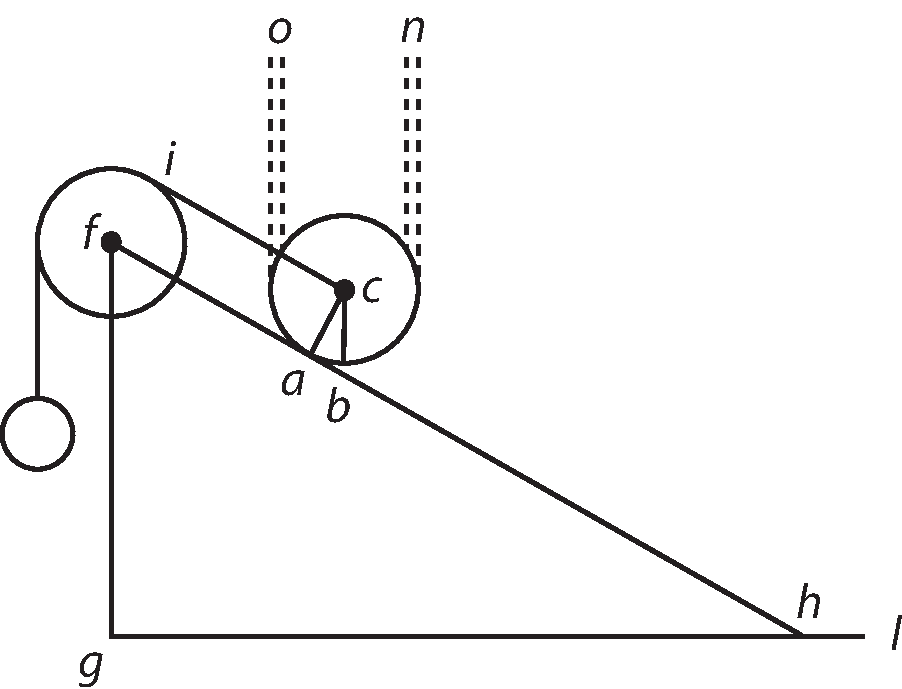
\includegraphics[width=0.47\textwidth]{images/lh0351402127r-1.pdf}\\
 \noindent \centering [\textit{Fig. 1}] 
\end{center}
\pend
\newpage
\pstart \noindent est totum, ratiocinantur de motu eodem \edtext{modo}{\lemma{modo}\Cfootnote{\textsc{I. G. Pardies}, \cite{00296}a.a.O., S. 82f.}} et n. 54 contra id quod ait des Cartes\protect\index{Namensregister}{\textso{Descartes} (Cartesius, des Cartes), Ren\'{e} 1596-1650}, corpus a quiete sua \edtext{sustineri. Si sint maxima duo corpora}{\lemma{sustineri.}\Bfootnote{\textit{(1)} Corpus \textit{(2)} Si corpus \textit{(3)} Si sint maxima duo corpora \textit{L}}} in bilance, \edtext{in aequilibrio, granum sabulis}{\lemma{bilance,}\Bfootnote{\textit{(1)} grani sabulis \textit{(2)} qu \textit{(3)} vince \textit{(4)} adj \textit{(5)} in aequilibrio, granum sabulis \textit{L}}} accedens faciet descendere alterum latus, et levabit oppositum, et quidem si incidat celeritate sua, inprimis (si aer non obstare \edtext{intelligatur).}{\lemma{intelligatur).}\Cfootnote{\textsc{I. G. Pardies}, \cite{00296}a.a.O., S. 88-92.}}
\pend 
\pstart%
\textso{60} Vis sans fin, est celle, \textit{qui engraine dans une roue à}
\edlabel{035,14,02_127r_a1}%
\edtext{}{{\xxref{035,14,02_127r_a1}{035,14,02_127r_a2}}{\lemma{\textit{dents.}}\Bfootnote{\textit{(1)} Le mouuement est tousjours pro \textit{(2)} \textso{61.} \textbar\ \textso{62} \textit{erg.} \textbar\ Quod motus est proportionalis \textit{L}}}}%
\edtext{\textit{dents.}}{\lemma{\textit{dents.}}\Cfootnote{\cite{00296}\textsc{I. G. Pardies}, a.a.O., S. 99.}}
\pend 
\count\Bfootins=1200
\count\Cfootins=1200
\pstart 
%\protect\begin{wrapfigure}{l}{0.3\textwidth}          
%\protect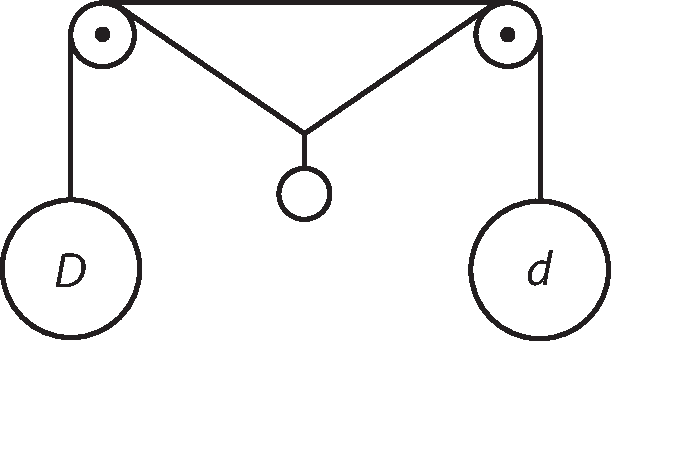
\includegraphics[width=0.3\textwidth]{images/lh0351402127r-2.pdf}
%\caption{Bildbeschreibung}
%\end{wrapfigure}
\textso{61.}
\textso{62}
Quod motus est proportionalis\edlabel{035,14,02_127r_a2} viribus,
%\pstart 
%\textso{60} Vis sans fin, est celle, \textit{qui engraine dans une roue a} \edtext{\textit{dents.}}{\lemma{\textit{dents.}}\Cfootnote{\cite{00296}\textsc{I. G. Pardies}, a.a.O., S. 99.}}
%\pend 
%\count\Bfootins=1200
%\count\Cfootins=1200
%\pstart 
%%\protect\begin{wrapfigure}{l}{0.3\textwidth}          
%%\protect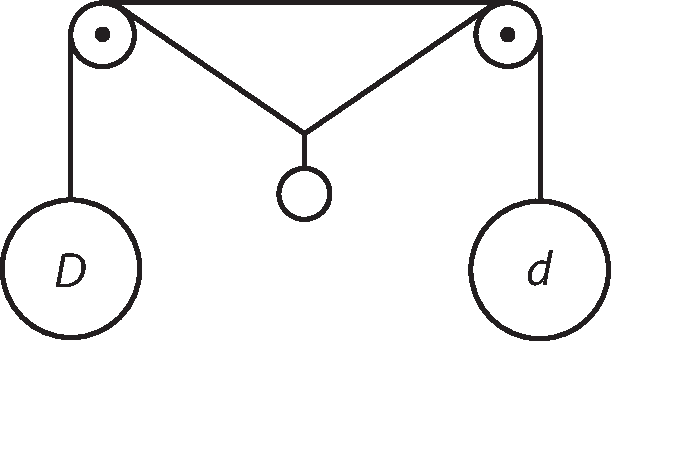
\includegraphics[width=0.3\textwidth]{images/lh0351402127r-2.pdf}
%%\caption{Bildbeschreibung}
%%\end{wrapfigure}
%\textso{61.} \edtext{\textso{62}}{\lemma{}\Bfootnote{\textso{62.} \textit{erg. L}}} \edtext{Quod motus est proportionalis}{\lemma{dents.}\Bfootnote{\textit{(1)} Le mouuement est tousjours pro \textit{(2)} \textso{61.} \textbar\ \textso{62.} \textit{erg.} \textbar\ Quod motus est proportionalis \textit{L}}} viribus, 
et quod majoribus opus non sit viribus ferendo corpori centum librarum in altitudinem pedis, vel \edtext{librae in altitudinem 100 pedum}{\lemma{librae}\Bfootnote{\textit{(1)} 100 librarum \textit{(2)} in altitudinem 100 pedum \textit{L}}}. Sed hoc non satisfacere animo, ut pro principio demonstrationum statui \edtext{queat.}{\lemma{queat.}\Cfootnote{\textsc{I. G. Pardies}, \cite{00296}a.a.O., S. 101f.}} Imo demonstratio quam ex Galilaeo\protect\index{Namensregister}{\textso{Galilei} (Galilaeus, Galileus), Galileo 1564-1642}
attulit non est \edtext{interna, et cogit non ostendit. Ut}{\lemma{interna,}\Bfootnote{\textit{(1)} sed e \textit{(2)} sed a \textit{(3)} et cogit non ostendit. Ut \textit{L}}} \textit{Geometriae Elementorum} Euclidis\protect\index{Namensregister}{\textso{Euklid} (Euclides) von Alexandria 287-212 v. Chr.}
in comparatione Geometriae indivisibilium. 
\pend 
\pstart \edtext{\textso{66-69} Utcunque magna pondera}{\lemma{\textso{66-69}.}\Bfootnote{\textit{(1)} Corpus \textit{(2)} Utcunque magna pondera \textit{L}}} \edtext{$d D$}{\lemma{$d D$}\Bfootnote{\textit{erg. L}}} suspendantur extremis chordae per duas trochleas incedentis, medium tamen pondus quantulumcunque nonnihil ea attrahet, seu chordam \edtext{attollet}{\lemma{attollet}\Cfootnote{\textsc{I. G. Pardies}, \cite{00296}a.a.O., S. 110f.}} ita etsi nullum sit pondus $e$ ipsum pondus chordae pro eo pot\-erit sumi, ideoque impossibile esse chordam qualiscunque viribus perfecte \edtext{tendere.}{\lemma{tendere.}\Cfootnote{\cite{00296}\textsc{I. G. Pardies}, a.a.O., S. 118f.}} Ego demonstrationem istam, esse puto paralogismum.
\pend
%\advanceline{-2}
\vspace*{2.5em}
\pstart
\begin{center}
  %\protect\begin{wrapfigure}{l}{0.3\textwidth}          
\noindent 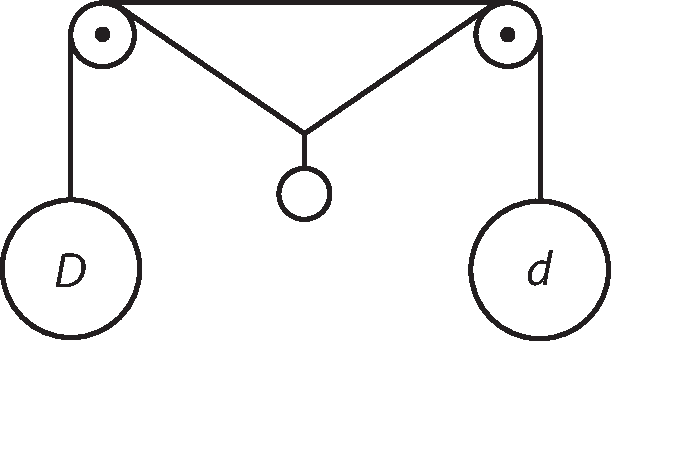
\includegraphics[trim = 0mm 10mm 0mm 0mm, clip, width=0.33\textwidth]{images/lh0351402127r-2.pdf}\\
\noindent \hspace{-8mm}[\textit{Fig. 2}] 
\end{center}
\pend
\count\Bfootins=1500
\count\Cfootins=1500
 


 

